\documentclass[a4j]{jarticle}

% \usepackage{showkeys}
\usepackage[dvips]{color,graphicx}
\usepackage{amsmath}
\usepackage{amssymb}
%\usepackage[utf8]{inputenc}
%\usepackage[T1]{fontenc}
%\usepackage{times}
%
\usepackage{amsmath,amssymb}
\usepackage{bm}
\usepackage{graphicx}
\usepackage{verbatim}
%
%\makeindex
%
%\setlength{\textwidth}{\fullwidth}
%\setlength{\textheight}{40\baselineskip}
\addtolength{\textheight}{\topskip}
\setlength{\voffset}{-0.55in}
%
\setcounter{tocdepth}{4}
\renewcommand{\contentsname}{\large \centerline{Contents}}

\def\thline{\noalign{\hrule height 1pt}}
%
\title{@Home SPLルールブック}
\author{Family \& Robotics Association}
\date{\today}

\begin{document}
%
%
\maketitle

\begin{center}
ルールに関する問い合わせ先: {\tt tc@familyrobotics.org}
\end{center}

\newpage
%
%
\tableofcontents
\newpage

\section{はじめに}

\subsection{このルールブックについて}

このルールブックは、RoboCup @Homeに標準ロボットリーグを
設ける提案及び、プレ競技会開催のために書かれるものである。
このルールブックの加筆修正・管理は、
Family \& Robotics AssociationのTechnical Comittee
(TC)によって行われる。

\section{ロボットの規格}

本リーグで使用するロボットは、家庭(主に日本国内の家庭)に
導入可能な大きさのものとして、TurtleBot2を用いる。

ハードウェアをワンメイクにする理由は、以下の通りである。
\begin{itemize}
	\item 各チームが同一の安価なハードウェアを用いる事によるハードウェア調達のコストを削減する。
	\item 組み立てやチューニングの手間の削減により、ソフトウェア開発を促進する。
\end{itemize}

\subsection{ロボットの構成}

ロボットは、台車、ロボットアーム、Kinect for Xbox 360、及び計算機で構成されることとする。
それらを動作させるための配線や基盤以外のものをロボットに搭載してはならない。

\subsubsection{台車、ロボットアーム}
台車、ロボットアームについては以下のものに限定する。
\begin{itemize}
	\item 台車: TurtleBot2\footnote{http://www.rt-shop.jp/index.php?main\_page=product\_info\&cPath=23\&products\_id=758}
	\item ロボットアーム: TurtleBot2用ロボットアーム``CRANE'' (クライン)あるいは``CRANE+''\footnote{http://www.rt-shop.jp/index.php?main\_page=product\_info\&cPath=1\&products\_id=1307}
\end{itemize}
これら商品は、取り扱い説明書の通りに正確に組み立てられていなければならない。

\subsubsection{ロボットに搭載する計算機}

計算機については、TurtleBot2のプレートに搭載するものとする。
最上段のプレートの上には置いてはならない。
計算機の個数の制限は設けない。寸法については、
プレートからの計算機筐体のはみ出しについて制限を設ける。
制限は、上面から見たときに、プレートの端から最も遠い部分が50[mm]
以内に収まっていなければならないというものとする。

\subsubsection{外部の計算機}

また、試技にはタブレットPCを利用するものがある。
この場合、ロボットに搭載された計算機からWiFiを通じて利用する。
WiFiのアクセスポイントはTCによって設置される
(\ref{sub:network}節参照)。

\section{環境}

\subsection{ロボットの行動する環境}\label{sub:environment}

%comment: なるべく簡素にしたほうがいいのか、@Homeの資材を使えるようにした方がよいのか・・・

競技は、一般家庭の部屋に見立てた環境で行われる。
環境の広さは$16$[m$^2$]以上とする。
この環境を、「リビング」と呼ぶ。
リビングは最低600[mm]の高さの白い光沢の無い壁で囲まれる。
消防法による制限がない場合は壁の代わりに建物の壁面を利用することがある。
この場合、白壁でない場合には、床から600[mm]以上の高さの白い紙を貼る。

床の材質は、TurtleBot2の走行に支障がないものとするが、
標準的なものは本ルールでは指定されない。
場合によってはカーペット等が設置されて数[mm]程度の段差が生じることがある。

リビングには、各試技において用いるテーブルや把持対象以外に、
飾りや障害物として食器棚や冷蔵庫等の什器が置かれることがある。

\subsection{通信環境と制限}\label{sub:network}

競技会では、
TCによりWiFiの公式アクセスポイント(公式AP)が準備される。

\subsubsection{接続できる計算機}

各チームが公式APとの接続できる計算機は、以下の通りである。

\begin{enumerate}
	\item ロボットに搭載された計算機
	\item 試技に用いるタブレット型(キーボードを持たない)PC
	\item 調整用の計算機
\end{enumerate}
IPアドレスの数は、IPアドレスが枯渇しない限りは特に制限を用いないが、
調整用の計算機は試技中には電源を切らなければならない。


\subsubsection{インターネットとの接続}

公式APは可能な場合、インターネットと接続されるが、
競技中は切断される。

\subsubsection{通信環境の責任の所在}

また、公式アクセスポイントの不具合に対する責任は
TCだけではなく各チームのリーダが負うことする。
競技中に遮断した場合については
リーダーミーティングで対応を行うこととする。
また、TCは通信機器を競技会に持ち込むことが
望ましいがこれは義務ではなく、TCからの要請があれば
競技会前に各チームのリーダーが中心となってチームからの
機器貸し出しの調整を行い、通信機器を準備しなければならない。


\section{試技}

%comment: 完全自律は難しいので半自律の試技を入れてみたがどうか。構成は半自律、自律、フリー演技

\subsection{試技1: これ取って来て}

試技1は、家庭においてロボットに欲しいものを
指示して取って来てもらうというタスクを想定して行う。
指示はタブレットPCやスマートフォンで行い、
タスク完了の有無、指示の量の多寡で評価を行う。

テーブルを二つ環境に用意し、図\ref{fig:test1}のように、
一方に操作者が座り、一方にロボットアームが把持できる物体をいくつか置く。
どの物体を運ぶかは審判から操作者に伝えられる。
ロボットが指定された物体を取り、
操作者のいるテーブルの上に置く。


\begin{figure}[h]
	\begin{center}
		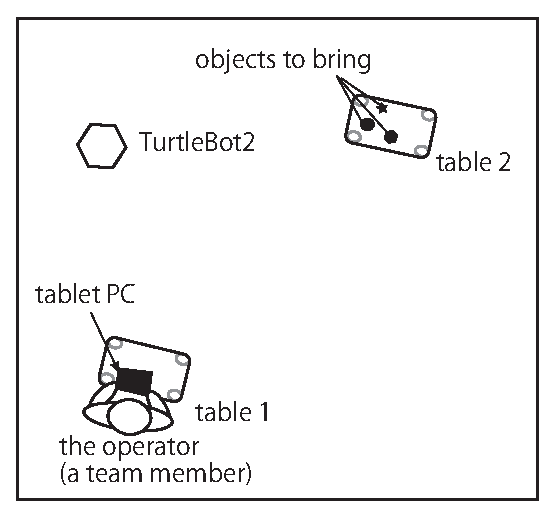
\includegraphics[width=0.4\linewidth]{./IMAGE/test1.eps}
		\caption{初期配置}
		\label{fig:test1}
	\end{center}
\end{figure}

%comment: 音声はどうしましょ?

\subsubsection{競技会前の準備}

物体については、あるメーカ製の消しゴム等、
日本国内で入手しやすいものとし、
競技会開催決定後、なるべく早い時点でTCが告知しなければならない。
リビングやテーブルの寸法については競技会会場で告知される。
テーブルの上に置く物体は$3$個から$5$個とする。

\subsubsection{試技前の準備}

テーブルや物体の具体的な配置は、
最初のチームが試技を行う直前にTCが決定する。
操作者の座る位置は操作者用のテーブルの周囲であればどこでもよいが、
後述のようにタブレットPCをテーブルに置ける距離でなければならない。

また、後に試技を行うチームが有利にならないように、各チームが
試技に用いるロボットとタブレットPCはTCが試技前に預かる。


\subsubsection{各チームの試技の流れ}

各チームに与えられる試技の時間は5[min]とする。
操作者は速やかにロボットとタブレットPCの準備を行う。
操作者と審判は、タブレットPCとロボットが通信を行える状態であることを確認する。
審判は操作者に準備完了の確認をとり、試技の開始を宣言する。
審判(2人以上)は、試技の経過時間と、
タブレット操作時間を計測する。
操作者は、タブレットPCを裏返してテーブルに置き、
手をタブレットから離すことで指示していないことを示す。
この時間は審判によって計測される。

指定された物体をテーブル以外の場所に落とした場合、
審判が試技を止める。この場合、
途中棄権した扱いで採点を行う。

\subsubsection{採点}

この試技では各チームの次の技術を評価する。
\begin{itemize}
	\item ロボットの自律あるいは半自律行動ソフトウェアのアイデアと実装
	\item タブレットPCやスマートフォンで使いやすいロボット操作アプリケーションのアイデアと実装
\end{itemize}
ロボットはなるべく自律行動を行うことが望ましく、
この場合に配点が最も高くなるが、
ロボットを操作するためのタブレットPCやスマートフォンの
アプリの開発に注力することにも一定の評価を与える。

以上の評価の方針を踏まえ、表\ref{table:test1score}のように配点を定める。


\begin{table}
\begin{center}
\caption{試技1の採点基準}
\label{table:test1score}
\begin{tabular}{l|p{5cm}|l|p{5cm}}
\thline
項目 & 条件 & 点数 & 備考\\
\hline
達成度 & 成功 & $+500$[点] & 成功すると、達成度は$500+500=1000$[点]となる。 \\
& 指定された物体にロボットアームで接触し、机からその物体が離れる(落下してもよい) & $+500$[点] \\
\hline
指示の量 & タブレットを裏返した時間& $+1$[点/s] & 秒以下の計測時間は切り捨て。試技が成功しないと与えられない。 \\
\hline
達成時間 & タスク成功後に残った時間 & $+1$[点/s] & 1秒以下の時間は切り捨て\\
\hline
反則等 & 試技中に操作者が立ってしまう & $-500$[点] & 床に足の裏以外の部分が接触してなければならない。何度でも減点される。 \\
	& ロボットがテーブルの天板以外の場所に物体を落とす & $-500$[点] & \\
\thline
\end{tabular}
\end{center}
\end{table}


\subsection{試技2: 片付け}

環境に箱と、それを片付ける場所があり、
ロボットは自律で動作し、箱を指定箇所に片付けなければならない。


図\ref{fig:test2}のように、箱、ロボット、収納場所、
障害物としてのテーブルがリビングに置かれる。
ロボットは箱を押して収納場所に箱を押し込む。

\begin{figure}[h]
	\begin{center}
		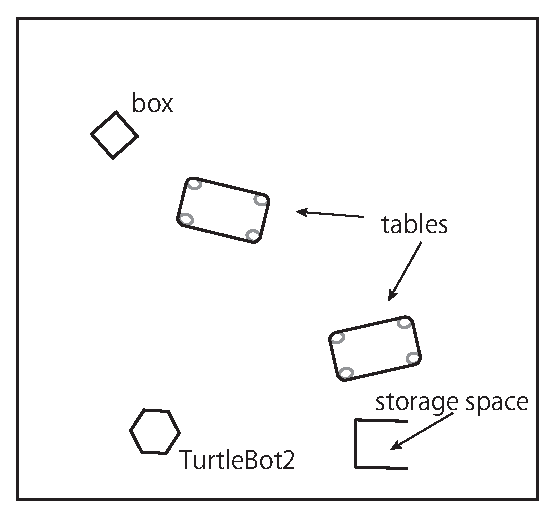
\includegraphics[width=0.4\linewidth]{./IMAGE/test2.eps}
		\caption{初期配置の例}
		\label{fig:test2}
	\end{center}
\end{figure}


箱は直方体で、一辺の長さが200[mm]以上、400[mm]以下とする。
また、TurtleBot2が押して運べる強度と軽さを持つものとする。
収納場所は、リビングに板でコの字型の領域を作り、その内部とする。
板は高さが500[mm]以上であり、箱が収まる大きさで作成される。


\subsubsection{試技の流れ}

ロボット、テーブル、箱、収納場所は、
試技2が開始される直前にTCによって決定され、
全チームが同じ初期配置から試技を開始する。
試技1同様、順番による有利不利が生じないように、
各チームのロボットはTCによって事前に集められる。

\subsubsection{採点}

この試技では、主に次の項目を評価することが意図されている。
\begin{itemize}
	\item ロボットによる環境の認識(地図生成等)
	\item 作成した地図からの大域的な動作計画と実行
	\item 箱の操作等の局所的な動作計画と実行
	\item 上記項目とは異なった、地図等に頼らない手法(創発的な手法等)
\end{itemize}

採点は、表\ref{table:test2score}の通り。

\begin{table}
\begin{center}
\caption{試技2の採点基準}
\label{table:test2score}
\begin{tabular}{l|p{5cm}|l|p{5cm}}
\thline
項目 & 条件 & 点数 & 備考\\
\hline
達成度 & 完全に終了 & $+700$[点] & 完全に終了で$300 + 700 = 1000$[点]となる \\
& 箱に触れる & $+300$[点] & \\
\hline
達成時間 & タスク成功後に残った時間 & $+1$[点/s] & 1秒以下の時間は切り捨て\\
\hline
不要な接触 & テーブルや壁、その他什器に触れる & $-200$[点] & 1回だけカウント\\
\thline
\end{tabular}
\end{center}
\end{table}


\subsection{試技3: フリー演技}

試技3は、各チームの技術力をアピールするためのフリー演技である。

\subsubsection{試技の流れ}

プレゼンテーション用のスクリーンと
プロジェクタがリビング横に設置される。
各チームには10分の試技時間が与えられ、
チームメンバーは試技時間中、
自由にプロジェクタとリビングを利用できる。
10分の試技は、次に述べる採点者によって採点される。
試技が終わるとすみやかに現状復帰を行い、
次のチームの準備に協力しなければならない。
この準備期間(前のチームの片付けと次のチームの準備)
には5分程度の時間を設ける。

\subsubsection{採点者}

参加チームメンバー、参加チーム関係者でない者から選出する。
TCメンバー、観客等から試技3の前に選出しておく。
採点者の人数は$3\sim10$人とする。
参加チーム関係者には、あるチームメンバーの大学・企業の同窓や、
指導教員、上司、親族、友人等が含まれる。
採点者に関係者が含まれているという疑いが生じた場合、
TCが試技3の順位を確定するまでにリーダーミーティングで
対応を協議する。
順位確定後は、明らかに関係者が含まれた場合においても
確定した順位が尊重される。
ただし、運営上可能である場合は、TCは順位確定を撤回し、
その関係者の点数を除いて再計算し、再確定することができる。

\subsubsection{採点者の途中離脱への対応}

一人の採点者の採点は、
その採点者が全チームの採点を終えた時点で有効となる。
つまり、途中で採点者が採点を放棄した場合、
あるいは採点を続行できなくなった場合、
その採点者の採点は無効となる。
TCは、有効な採点者の人数が$3$人を割り込まないように、
事前にその旨をTC以外の採点者に告知しなければならない。
万が一、採点者数が$3$人を割り込む場合、
リーダーミーティングにおいて採点方法を決める。

\subsubsection{採点基準}

一人の採点者は、表\ref{table:test3score}の採点表に従って採点を行う。
採点表のように、各チームには、ただロボットを動かすだけではなく、
採点者や観客に自らの意図を伝えることが求められる。


\begin{table}
\begin{center}
\caption{試技3の採点基準}
\label{table:test3score}
\begin{tabular}{l|p{4cm}|l|p{4cm}}
\thline
項目 & 条件 & 点数 & 備考\\
\hline
問題設定 & 興味を引くタスクか。家庭での実用を狙っているか。 & $0\sim100$[点] & 主観でよい。\\
\hline
達成度 & チームメンバーがやると言ったタスクをロボットがやり遂げたか。 & $0\sim100$[点] & タスクが曖昧な場合は厳しく採点すること。 \\
\hline
技術 & 技術的な新規性があるか。難易度があるか。 & $0\sim100$[点]  & 新規性、難易度のどちらかがあればよい。\\
\hline
プレゼンテーション & 説明が適切か。退屈しないか。 & $0\sim100$[点] & 主観でよい。\\
\hline
後始末 & 現状復帰できているか。 & $-100$[点] & 次のチームに迷惑をかけた場合、採点者が注意する。注意した内容が達成できない場合に$100$点を減点。\\
\thline
\end{tabular}
\end{center}
\end{table}



\section{競技会での順位}

\subsection{順位の決定}

競技会における順位は、次のように決定される。
TCは、チーム数や棄権チーム数を勘案し、
優勝からある順位までを表彰するかを競技会に決定する。

\subsubsection{各試技の順位点}\label{sub:testrank}

競技会への登録チーム数\footnote{試技への登録チーム数ではないことに注意}を$m$とする。
あるチームの、その試技での得点が上から$n$番目に高いとき、
このチームの、その試技における順位点を
\[
	m - n + 1
\]
点と定義する。つまり、その試技で$1$位であれば$m$点、最下位であれば$1$点となる。
また、試技を棄権した場合には$0$点となる。

また、複数のチームの得点が一緒で$n$位タイであった場合、
同点のチーム数が$\ell$のとき、次のように順位点を計算する。
\[
	\dfrac{\sum_{i=0}^{\ell-1}(n + i)}{\ell}
\]
つまり、4位タイが3チームであれば$(4+5+6)/3=5$[点]ということである。


\subsection{競技会での順位}

各試技の「順位点」の合計で決定する。順位点が同点の場合、
試技3のフリー演技の順位の優劣で順位を決定する。
試技3が同順位の場合は試技2、それも同順位なら試技1の順位で決定する。
試技がすべて同着であれば、同順とする。
例えば、2チームが全く同じ点数で3つの試技を終え、
順位点の合計で4位タイだとすれば、そのまま4位として扱う。
1位タイの場合は両チーム1位としてよい。
ただし、過半数のチームが1位等、賞の希少性を損ねる結果になった場合には、
表彰されない場合があり、その場合の裁定については、
TCが行う。

\subsection{その他表彰}

\subsubsection{Family \& Robotics賞}

競技会において技術的な新規性、有用性、学術性、
その他特異性が最も顕著であったチームを
TCが1チーム選出し、「Family \& Robotics賞」を与える。
責任者となったTCメンバーは賞の候補チームを選び、
チームから簡単なヒアリング(立ち話程度でよい)
を行って1チームを選出する。

選出にあたっては、競技会での高順位チームよりも、
下位で目立ったチームを優先することとする。
これは、以下の理由があってのことである。
\begin{itemize}
	\item 高順位のチームはその順位で技術力を既に評価されていること。
	\item 技術的な多様性を保つためにユニークな発想を優遇しなければならない。
\end{itemize}

\subsubsection{他団体からの表彰}

他団体からの表彰の申し入れがあった場合、TCが対応する。
積極的に受け入れることとする。

\section{その他}

\subsection{試技における審判}

審判は、チームメンバーが担当することとする。
試技を行うチームのメンバーが、そのチームの
審判を行うことはできない。

\subsection{大会期間中におけるリーダーミーティングの設置}

本リーグは、各チームが主体的に運営することとし、
競技会中は、全チームのリーダーが集まったリーダーミーティングが
最も重要な組織である。
リーダーミーティングの議決は本書のルールの
一時的な改変等、ほぼ全ての事項について効力を発揮する。
ただし、効力の発揮にはTCの了承が必要である。
また、議決の方法も
リーダーミーティングにおいて決定されなければならない。


一時的な改変を積極的に行うべき例としては、以下があげられる。
\begin{itemize}
	\item 各試技のルールが全チームに対して厳しすぎる。
	\item 試技1のように操作者がいる場合で、操作者に障碍がある。
\end{itemize}
いずれも競技会を盛り上げ、円滑に運営するために柔軟な対応が求められる。

\subsubsection{ルール読み合わせの義務}

また、ルールに関するトラブルを避けるため、
競技前にリーダーミーティングにおいてルールの
読み合わせが行われなければならない。

\subsubsection{リーダー以外の参加者}

リーダーミーティングには、リーダーでない一般メンバー、TC
もオブザーバーとして参加できる。
また、出席の求めがあった場合、
指名された一般メンバーは参加しなくてはならない。

\subsubsection{開催のタイミング}

競技中のトラブルの発生、あるチームの不正疑惑等が発生した場合、
TCメンバー、あるいはチームリーダーは、
他のチームリーダーに呼びかけてリーダーミーティングを開催する事ができる。
ただし、緊急を要するもの以外は、
観客が入っている時間帯を極力さけるものとする。

\subsection{コードの公開}

TCの指定する競技会においては、出場したチームは
使用したコード(ロボット上の計算機内で使用した自作、流用コード・
タブレット等の操作用プログラム)を公開する義務を負う。
公開先については、TCの管理効率化の観点からGitHubが望ましい。
公開したら、速やかにTCに電子メールで連絡する。


ソフトウェア公開には以下の意図がある。
\begin{itemize}
	\item 有力チームの連続優勝を困難にする。
	\item リーグ全体の技術力向上を促進する。
	\item 新規参入の障壁を下げる。
	\item 参加者がオープンソース文化に親しむ。
\end{itemize}
公開の無いチームは、次の競技会への参加が許可されない。

\subsubsection{ライセンスの制限}

ライセンスについては、様々な議論が存在するが、
本競技会においてはMITライセンス等
BSDスタイルのライセンスを選択することとする。
公開の義務はコードではなく大会参加資格の取得のために発生することとし、
コード自体への公開義務を避けることとする。

特にGPLに関しては、
下記\ref{sub:licence_exception}項が適用されるチームが不利益を被るため、
継続して@Home SPLに参加する場合には選択はできないこととなる。
また、GPLのコードがチームのコードに混入すると、
BSDスタイルのライセンスが適用できなくなるため、
十分に注意すること。

\subsubsection{公開に関する例外}\label{sub:licence_exception}

資金提供者との利害関係がある場合、あるいは特許出願・ビジネスのための
コードが含まれ、公開が困難な場合は、
その機能の実装部分を非公開とすることができる。
また、その旨はREADME等、分かりやすい場所に明記する必要がある。
コード全体を非公開とすることはできず、
非公開とする部分とのインタフェースが分かるコードが
公開されなければならない。


コードの非公開は、500日を超えて行うことはできない。
例えば、ある年次大会で使用して非公開としたコードについては、
その翌々年の大会には使用できない。
あるいは、使用したら公開しなければならない。
当該コードを使用しない場合、公開できる代替のコードを使わなければならない。

\subsubsection{不正の処分}


コード公開に関する不正については、
事後に明らかになると考えられ、
その場合、優勝の取り消し等、
リーグからネガティブな事項の公表を行う必要が発生する。
そのため、コード公開に関する不正があったチームは、
永久追放、その旨の公示等、厳罰に処される。

%
\end{document}
